\subsection{Упражнение 1}

Выясним, что случится, при увеличении ширины Гауссова окна std не увеличивая ширину окна m

Функция расширения массива нулями

\begin{lstlisting}[language=Python]
from thinkdsp import SquareSignal
from thinkdsp import decorate

def zero_pad(array, n):
    """Extends an array with zeros.

    array: NumPy array
    n: length of result

    returns: new NumPy array
    """
    res = np.zeros(n)
    res[:len(array)] = array
    return res


def plot_filter(M=11, std=2):
    signal = SquareSignal(freq=440)
    wave = signal.make_wave(duration=1, framerate=44100)
    spectrum = wave.make_spectrum()

    gaussian = scipy.signal.gaussian(M=M, std=std)
    gaussian /= sum(gaussian)

    ys = np.convolve(wave.ys, gaussian, mode='same')
    smooth =  Wave(ys, framerate=wave.framerate)
    spectrum2 = smooth.make_spectrum()

    # plot the ratio of the original and smoothed spectrum
    amps = spectrum.amps
    amps2 = spectrum2.amps
    ratio = amps2 / amps    
    ratio[amps<560] = 0

    # plot the same ratio along with the FFT of the window
    padded =  zero_pad(gaussian, len(wave))
    dft_gaussian = np.fft.rfft(padded)

    plt.plot(np.abs(dft_gaussian), color='gray', label='Gaussian filter')
    plt.plot(ratio, label='amplitude ratio')

    decorate(xlabel='Frequency (Hz)', ylabel='Amplitude ratio')
    plt.show()
    
\end{lstlisting}

\begin{lstlisting}[language=Python]
from ipywidgets import interact, interactive, fixed
import ipywidgets as widgets
from thinkdsp import Wave
import scipy.signal

slider = widgets.IntSlider(min=2, max=100, value=11)
slider2 = widgets.FloatSlider(min=0, max=20, value=2)
interact(plot_filter, M=slider, std=slider2);
\end{lstlisting}

\begin{figure}[H]
	\begin{center}
		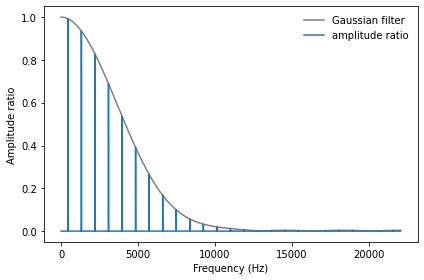
\includegraphics[scale=1]{fig/lab08/lab08_01.png}
		\caption{Гауссово окно для фильтрации}
	\end{center}
\end{figure}

\begin{lstlisting}[language=Python]
gaussian = scipy.signal.gaussian(M=11, std=11)
gaussian /= sum(gaussian)

plt.plot(gaussian, label='Gaussian')
decorate(xlabel='Index')
\end{lstlisting}

\begin{figure}[H]
	\begin{center}
		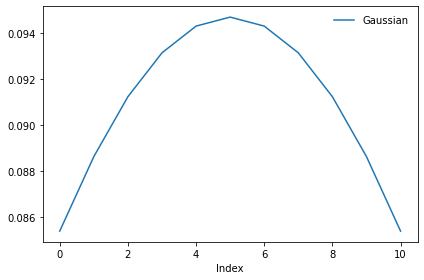
\includegraphics[scale=0.7]{fig/lab08/lab08_02.png}
		\caption{Гауссово окно}
	\end{center}
\end{figure}

\begin{lstlisting}[language=Python]
gaussian = scipy.signal.gaussian(M=11, std=1000)
gaussian /= sum(gaussian)

plt.plot(gaussian, label='Gaussian')
decorate(xlabel='Index')
\end{lstlisting}

\begin{figure}[H]
	\begin{center}
		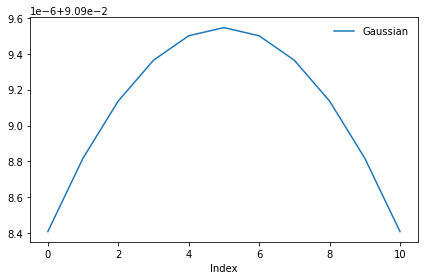
\includegraphics[scale=0.7]{fig/lab08/lab08_03.png}
		\caption{Гауссово окно}
	\end{center}
\end{figure}

Исходя из результатов видно, что при увеличении std -> кривая становится шире, а сам БПФ меньше (уже).


\subsection{Упражнение 2}

Протестируем, является ли преобразование Фурье гауссовой кривой - также гауссовой кривой.

Кривая Гаусса

\begin{lstlisting}[language=Python]
gaussian = scipy.signal.gaussian(M=32, std=2)
gaussian /= sum(gaussian)

plt.plot(gaussian, label='Gaussian')
decorate(xlabel='Index')
\end{lstlisting}

\begin{figure}[H]
	\begin{center}
		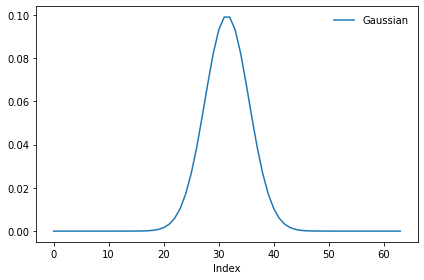
\includegraphics[scale=0.7]{fig/lab08/lab08_04.png}
		\caption{Гауссово окно}
	\end{center}
\end{figure}

Применим БПФ

\begin{lstlisting}[language=Python]
fft_gaussian = np.fft.fft(gaussian)
plt.plot(abs(fft_gaussian), label='Gaussian')
\end{lstlisting}
\begin{figure}[H]
	\begin{center}
		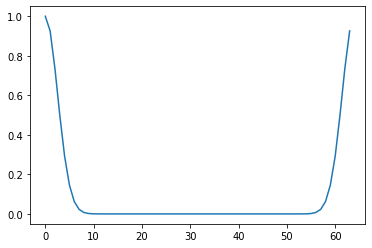
\includegraphics[scale=1]{fig/lab08/lab08_05.png}
		\caption{FTT применённое на окно}
	\end{center}
\end{figure}

Произведем свертку отрицательных частот влево.

\begin{lstlisting}[language=Python]
fft_rolled_gaussian = np.roll(fft_gaussian, len(gaussian) // 2)
plt.plot(abs(fft_rolled_gaussian), label='Gaussian')
\end{lstlisting}
\begin{figure}[H]
	\begin{center}
		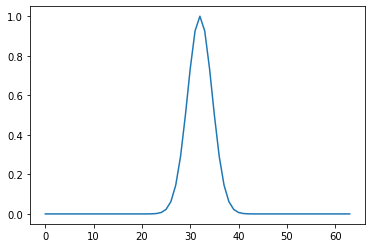
\includegraphics[scale=1]{fig/lab08/lab08_06.png}
		\caption{Результат}
	\end{center}
\end{figure}

Преобразование Фурье гауссовой кривой приблизительно похоже на гауссову кривую


\subsection{Упражнение 3}

Поэксперементируем с окнами, поищем подходящее для НЧ

\begin{lstlisting}[language=Python]
signal = SquareSignal(freq=220)
wave = signal.make_wave(duration=1, framerate=44100)

M = 8
std = 2

gaussian = scipy.signal.gaussian(M=M, std=std)
blackman = np.blackman(M)
bartlett = np.bartlett(M)
hanning = np.hanning(M)
hamming= np.hamming(M)

windows  = [gaussian, blackman, bartlett, hanning, hamming]
labels = ['gaussian','blackman','bartlett','hanning','hamming']

for element, label in zip(windows,labels):
    element /= sum(element)
    plt.plot(element,label=label)
    
plt.legend()
\end{lstlisting}

Построим графики для нескольких окон

\begin{figure}[H]
	\begin{center}
		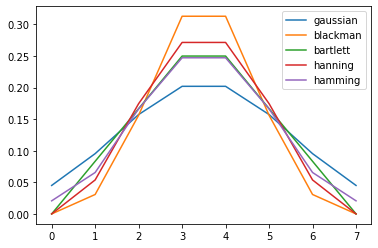
\includegraphics[scale=1]{fig/lab08/lab08_07.png}
		\caption{Применение различных окон на выбранный сигнал}
	\end{center}
\end{figure}

Графики дикретного преобразования Фурье

\begin{lstlisting}[language=Python]
for element, label in zip(windows, labels):
    padded =  zero_pad(element, len(wave))
    dft_window = np.fft.rfft(padded)
    plt.plot(abs(dft_window), label=label)
    
plt.legend()
\end{lstlisting}

\begin{figure}[H]
	\begin{center}
		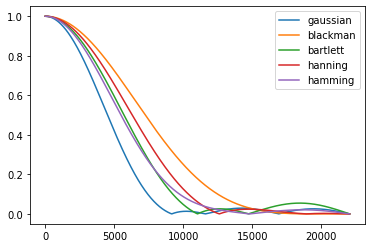
\includegraphics[scale=1]{fig/lab08/lab08_08.png}
		\caption{Применение различных окон на выбранный сигнал}
	\end{center}
\end{figure}

\begin{lstlisting}[language=Python]
for element, label in zip(windows, labels):
    padded =  zero_pad(element, len(wave))
    dft_window = np.fft.rfft(padded)
    plt.plot(abs(dft_window), label=label)

plt.legend()
decorate(yscale='log')
\end{lstlisting}

\begin{figure}[H]
	\begin{center}
		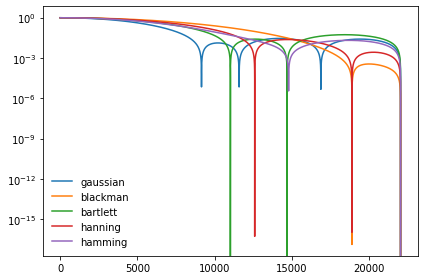
\includegraphics[scale=1]{fig/lab08/lab08_09.png}
		\caption{Применение различных окон на выбранный сигнал в лагорифмическом масштабе}
	\end{center}
\end{figure}

Исходя из этого и предыдущих графиков можно сделать вывод, что Хэнинг лучше всего подоёдет для фильтрации низких частот за счет быстрого спада и минимальных боковых лепестков.


\subsection{Вывод}

В данной работе были рассмотрены фильтрации, свёртки, сглаживания. Сглаживание - операция удаляющая быстрые изменения сигнала для выявления общих особенностей. Свёртка - применение оконной функции к перекрывающимся сигментам сигнала. В упражнениях были исследованы различные свойства данных явлений.
